%
% main.tex -- Paper zum Thema <resultante>
%
% (c) 2026 Jakob Gierer, OST Ostschweizer Fachhochschule
%
% !TEX root = ../../buch.tex
% !TEX encoding = UTF-8
%
\chapter{Gemeinsame Nullstellen und Resultante\label{chapter:resultante}}
\kopflinks{Gemeinsame Nullstellen und Resultante}
\begin{refsection}
\chapterauthor{Jakob Gierer}
\index{Jakob Gierer}%
\index{Gierer, Jakob}%

%
% 0_Einleitung.tex -- Einleitung zum Kapitel Resultante
%
% (c) 2026 Jakob Gierer, OST Ostschweizer Fachhochschule
%
% !TEX root = ../../buch.tex
% !TEX encoding = UTF-8
%
\section{Einleitung\label{resultante:section:einleitung}}
\kopfrechts{Einleitung}

Für die Lösung von Integralen greifen Ingenieur:innen sowie Studierende oft auf Computeralgebrasysteme (CAS) zurück.
\index{Computeralgebrasystem}%
Damit CAS-fähige Rechner Integrale lösen können, werden effiziente Algorithmen benötigt.
Integranden werden zunächst in einen polynomiellen Teil und einen rationalen Teil aufgeteilt.
Dieses Kapitel behandelt nur Methoden zur Bestimmung der Stammfunktion des rationalen Teils.
Dabei besteht der rationale Teil des Integrals aus echt gebrochenen Funktionen. 
Für die Berechnung dieser Integrale müssen die Nullstellen des Nennerpolynoms der Integranden bestimmt werden.

In Abschnitt \ref{buch:ratint:section:rothsteintrager} wird der Satz von Rothstein-Trager beschrieben, der für die Bestimmung der Nullstellen in Kapitel \ref{chapter:intalg} den euklidischen Algorithmus nutzt.
\index{Rothstein-Trager, Satz von}%
\index{Satz!von Rothstein-Trager}%
In diesem Kapitel soll eine weitere Methode zur Berechnung von Nullstellen vorgestellt werden, die Resultante.
In verschiedenen Lehrbüchern wird die Resultante als
\begin{equation}
    \Res(f,g)=\det(\syl(f,g))
    \label{resultante:equation:definition}
\end{equation}
definiert. Aber was ist \(\syl\)? 
Und was ist die Resultante?

Was genau die Resultante ist und welche nützlichen Eigenschaften sie hat, beschreibt dieses Kapitel.
Die Beschreibungen und Ideen in diesem Kapitel basieren auf \cite{resultante:Linalg} und \cite{resultante:SymInt}.

%
% 1_Idee.tex -- Abschnitt 1 Grundidee der Sylvester-Matrix
%
% (c) 2026 Jakob Gierer, OST Ostschweizer Fachhochschule
%
% !TEX root = ../../buch.tex
% !TEX encoding = UTF-8
%
\section{Grundlegende Idee
\label{resultante:section:Idee}}
\kopfrechts{Grundlegende Idee}
Haben die Polynome \(f(X)=f_mX^m+\dots+f_1X+f_0\) mit \(\deg(f)=m\)
und \(g(X)=g_nX^n+\dots+g_1X+g_0\) mit \(\deg(g)=n\) einen gemeinsamen
Teiler \(d(X)\), dessen Grad mindestens \(1\) ist?

\noindent
Falls ja, dann gibt es Polynome \(p(X)\) und \(q(X)\) mit
\begin{equation}
    f(X)=q(X)\cdot d(X)\quad \text{und} \quad
    g(X)=p(X)\cdot d(X)
    \label{resultante:equation:divisor}
\end{equation}
mit \(\deg (d) \geq 1\), \(\deg(q)<\deg(f)\) und \(\deg(p)<\deg(g)\).

Aus (\ref{resultante:equation:divisor}) folgt
\begin{equation}
    \deg (q) = \deg (f) - \deg (d) \leq m-1 \quad \text{und} \quad
    \deg (p) = \deg (g) - \deg (d) \leq n-1.
\end{equation}
Das Polynom (\ref{resultante:equation:divisor}) links wird mit \(p(X)\)
multipliziert und das Polynom (\ref{resultante:equation:divisor}) rechts
mit \(q(X)\).
Aus diesen erweiterten Polynomen wird die Differenz
\begin{equation}
    fp-gq=0
    \label{resultante:equation:lgs}
\end{equation}
gebildet.
Daraus lässt sich eine Gleichung für die Koeffizienten von \(p\)
und \(q\) gewinnen.
Da der Grad von \(d(X)\) vorher nicht bekannt ist, wird hier mit dem
kleinsten Grad von \(d(X)\) weiterverfahren.
Sollte \(\deg d(X)=2\) sein, so werden die höchsten Koeffizienten von
\(q(X)\) und \(p(X)\) einfach \(0\).
\begin{figure}
    \centering
    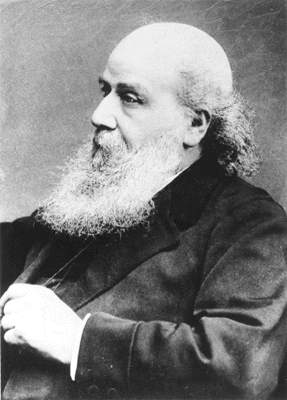
\includegraphics[width=0.4\textwidth]{papers/resultante/pictures/jjsylvester.png}
    \caption{Der britische Mathematiker James Joseph Sylvester \cite{resultante:jjsylvester}.}
\index{Sylvester, James Joseph}%
    \label{resultante:fig:jjsylvester}
\end{figure}
\begin{beispiel}
    Für die Polynome \(f(X)=2X^3+7X^2-5X-4\) und \(g(X)=2X^2+X-3\) werden
    die um Grad \(1\) kleineren Hilfspolynome \(q(X)=q_2X^2+q_1X+q_0\)
    und \(p(X)=p_1X+p_0\) bestimmt.
    Diese werden nun in (\ref{resultante:equation:lgs}) eingesetzt und
    nach den Koeffizienten absteigend sortiert, daraus resultiert die
    Polynomgleichung
    \begin{equation}
        \begin{aligned}
            (2p_1-2q_2)& X^4+\\
            (7p_1+2p_0-q_2-2q_1)& X^3+\\
            (-5p_1+7p_0+3q_2-q_1-2q_0)& X^2+\\
            (-4p_1-5p_0+3q_1-q_0)& X^{\phantom{0}}+\\
            (-4p_0+3q_0)& \phantom{X^0}=0.
        \end{aligned}
        \label{resultante:equation:gs}
    \end{equation}
    Dass in (\ref{resultante:equation:gs}) alle Koeffizienten
    verschwinden, kann als Gleichungssystem in der Matrixform
    \begin{equation}
        \begin{pmatrix}
            p_1&p_0&-q_2&-q_1&-q_0
        \end{pmatrix}
        \,
        \begin{pmatrix*}[r]
            2 &\phantom{-}7 & -5 & -4 &  0 \\
            0 &           2 &  7 & -5 & -4 \\
            2 &           1 & -3 &  0 &  0 \\
            0 &           2 &  1 & -3 &  0 \\
            0 &           0 &  2 &  1 & -3
        \end{pmatrix*}=0
        \label{resultante:equation:Syl}
    \end{equation}
    für die Koeffizienten der Hilfspolynome \(q(X)\) und
    \(p(X)\) geschrieben werden. Die Systemmatrix der Gleichung
    (\ref{resultante:equation:Syl}) ist die Sylvester-Matrix,
    benannt nach dem britischen Mathematiker James Joseph Sylvester
    (Abb.~\ref{resultante:fig:jjsylvester}).
    \label{resultante:beispiel:lgs}
\end{beispiel}
Die Idee der Umformungsschritte bis hierher ist, eine Übersicht zu
bekommen, woher die Sylvester-Matrix kommt.

\subsection{Die Sylvester-Matrix
\label{resultante:subsection:Sylvester-Matrix}}
Für zwei Polynome kann die in (\ref{resultante:equation:Syl}) gefundene
Matrix wie folgt allgemein definiert werden.

\begin{definition}[Sylvester-Matrix]
\index{Sylvester-Matrix}%
    Seien \(a(X)=a_nX^n+a_{n-1}X^{n-1}+\dots+a_1X+a_0\) und
    \(b(X)=b_mX^m+b_{m-1}X^{m-1}+\dots+b_1X+b_0\) Polynome vom Grad
    \(\deg a=n\) beziehungsweise \(\deg b=m\).
    Die \emph{Sylvester-Matrix} von a und b ist die \((n + m) \times
    (n + m)\)-Matrix:
    % \begin{equation}
        
    %     \begin{pmatrix}
    %         a_n&a_{n-1}&a_{n-2}&\dots&&&&&\\
    %         &a_n&a_{n-1}&a_{n-2}&\dots&&&&\\ 
    %         &&a_n&a_{n-1}&a_{n-2}&\dots&&&\\
    %         &&&\ddots&\ddots&\ddots&\ddots&&\\
    %         &&&&&\dots&a_1&a_0&\\
    %         &&&&&&\dots&a_1&a_0\\ \hdashline
    %         b_m&b_{m-1}&b_{m-2}&\dots&&&&&\\
    %         &b_m&b_{m-1}&b_{m-2}&\dots&&&&\\ 
    %         &&b_m&b_{m-1}&b_{m-2}&\dots&&&\\
    %         &&&\ddots&\ddots&\ddots&\ddots&&\\
    %         &&&&&\dots&b_1&b_0&\\
    %         &&&&&&\dots&b_1&b_0\\
    %     \end{pmatrix}
    % \end{equation}
    \NiceMatrixOptions
    {
        custom-line ={command= H, tikz= dashed, width= \pgflinewidth}, % horizontal, dashed
    }
    \begin{equation*}
        \syl(a,b)=
        \begin{pNiceMatrix}[last-col,extra-margin=4pt]
            a_n&a_{n-1}&a_{n-2}&\dots&&&&&
            &\Block{6-1}{\hspace*{11pt}m\text{-Zeilen}}\\
            &a_n&a_{n-1}&a_{n-2}&\dots&&&&&\\ 
            &&a_n&a_{n-1}&a_{n-2}&\dots&&&&\\
            &&&\ddots&\ddots&\ddots&\ddots&&&\\
            &&&&&\dots&a_1&a_0&&\\
            &&&&&&\dots&a_1&a_0&\\
            \H
            b_m&b_{m-1}&b_{m-2}&\dots&&&&&
            &\Block{6-1}{\hspace*{11pt}n\text{-Zeilen}}\\
            &b_m&b_{m-1}&b_{m-2}&\dots&&&&&\\ 
            &&b_m&b_{m-1}&b_{m-2}&\dots&&&&\\
            &&&\ddots&\ddots&\ddots&\ddots&&&\\
            &&&&&\dots&b_1&b_0&&\\
            &&&&&&\dots&b_1&b_0&\\
            \CodeAfter
            \SubMatrix{.}{1-1}{6-9}{\}}[right-xshift=9pt]
            \SubMatrix{.}{7-1}{12-9}{\}}[right-xshift=9pt]
        \end{pNiceMatrix},
        \label{resultante:equation:Syldef}
    \end{equation*}
wobei die Koeffizienten von \(a(X)\) \(m\)-mal und die von \(b(X)\)
\(n\)-mal wiederholt werden.
\label{resultante:definition:Sylvester}
\end{definition}

Wie sich in der Herleitung (\ref{resultante:equation:Syl}) und der
Definition \ref{resultante:definition:Sylvester} der Sylvester-Matrix
beobachten lässt, kann die Sylvester-Matrix gebildet werden, indem man
die Koeffizienten des Polynoms \(a(X)\) so oft wiederholt, wie der Grad
\(\deg(b)=m\) angibt.
Analog dazu wird mit dem Polynom \(b(X)\) verfahren.

Die eigentliche Idee der Sylvester-Matrix ist, das algebraische
Problem: ``Haben zwei Polynome einen gemeinsamen Faktor?'', in das
lineare Problem: ``Sind zwei bestimmt verschobene Polynome linear
abhängig?'' umzuformulieren.
Diese Umformung wird später in diesem Kapitel für die Definition
\ref{resultante:definition:resultante} wichtig.

%
% 2_ggT.tex -- Abschnitt 2 ggT berechnung mit der Tableau Methode
%
% (c) 2026 Jakob Gierer, OST Ostschweizer Fachhochschule
%
% !TEX root = ../../buch.tex
% !TEX encoding = UTF-8
%
\section{Grösster gemeinsamer Teiler (ggT)
\label{resultante:section:ggT}}
\kopfrechts{Grösster gemeinsamer Teiler}
\subsubsection{ggT in der Tableau-Methode
\label{resultante:subsubsection:tableau}}
Die Tableau-Methode entsteht aus dem euklidischen Algorithmus, für den
\index{euklidischer Algorithmus}%
man die Polynomdivision als Tableau schreibt.
\index{Polynomdivision}%
Die Berechnung des grössten gemeinsamen Teilers von \(a(X)\) und \(b(X)\)
mit \(n = \deg (a) \geq m = \deg (b)\) in der Tableau-Methode beginnt
mit der Sylvester-Matrix \(\syl(b,a)\).
Das ist die Matrix aus Definition \ref{resultante:definition:Sylvester},
in der alle \(m\) Zeilen des \(a(X)\)-Polynoms mit denen des
\(b(X)\)-Polynoms vertauscht werden.
Auf diese Matrix werden nun \(n-m+1\)-Gauss-Zeilenoperationen angewandt.
Die Zeilenoperationen führen im Wesentlichen zu einer Polynomdivision,
\index{Zeilenoperation}%
wie das der euklidische Algorithmus ebenfalls macht.
In den unteren \(m\) Zeilen, an der Stelle der \(a(X)\)-Polynome, entsteht
der entsprechende Rest \(r(X)\) (grüne Zeilen) der Division von \(a(X)\)
und \(b(X)\).
Um nun auf die Stufenform der Sylvester-Matrix zurück zu kommen,
\index{Stufenform}%
werden auf den Restpolynomen zusätzliche Zeilenoperationen angewandt,
bis der Rest sich auf jeder Zeile wiederholt.
Des Weiteren enthalten die ersten \(n-m+1\) Spalten Nullen:
\begin{equation*}
    \centering
    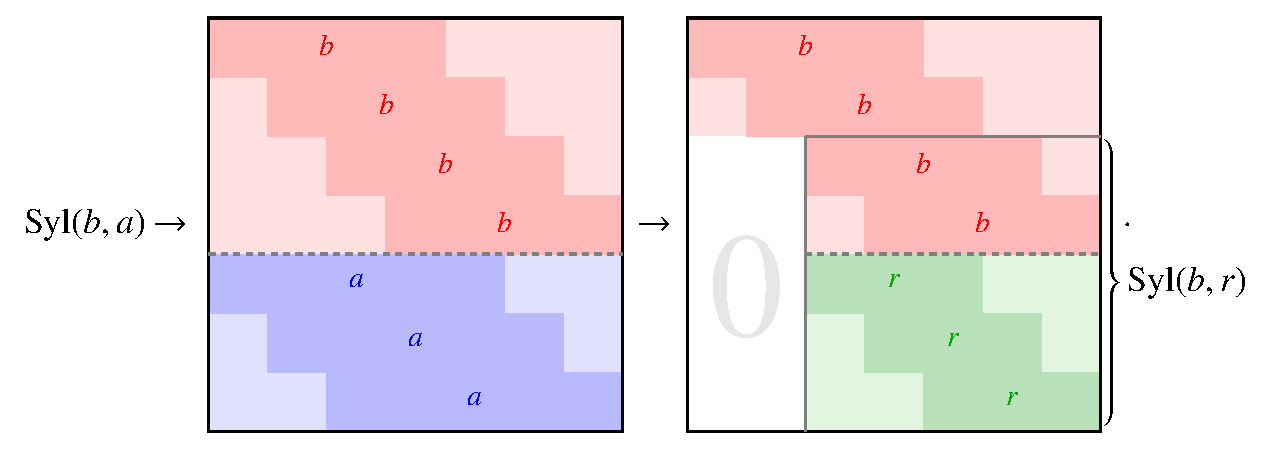
\includegraphics[width=\textwidth]{papers/resultante/pictures/SylvesterTableau.pdf}
    \label{resultante:equation:sylvesterTab}
\end{equation*}
In der rechten unteren Ecke ist nun eine kleinere Sylvester-Matrix
\(\syl(b,r)\) entstanden.
Die Polynome in der neuen Sylvester-Matrix werden ebenfalls vertauscht,
dann kann der nächste Rest mit derselben Methode berechnet werden.
Das zeigt das folgende Beispiel.

\begin{beispiel}
    Die Vorgehensweise zur Ermittlung des grössten gemeinsamen
    Teilers wird am Beispiel \(a(X)=4X^4-7X^3+22X^2-24X+5\) und
    \(b(X)=8X^3+8X^2-16X\) gezeigt.
    Im ersten Tableau sind die ersten vier Zeilen Kopien von \(b(X)\)
    und die drei darunter liegenden sind Kopien von \(a(X)\):
    \begin{equation*}
	\def\r#1{\bgroup\color{darkred}#1\egroup}
	\def\b#1{\bgroup\color{blue}#1\egroup}
	\def\g#1{\bgroup\color{darkgreen}#1\egroup}
	\def\l#1{\bgroup\color{gray!20}#1\egroup}
	\def\p{\phantom{-}}
        \begin{NiceArray}{*{7}{r}}[cell-space-limits=3pt]
        \r{8} & \r{8}  & \r{-16} & \r{0}   & \l{0}   & \l{0}   & \p\l{0} \\
        \l{0} & \r{8}  & \r{8}   & \r{-16} & \r{0}   & \l{0}   & \l{0} \\
        \l{0} & \l{0}  & \r{8}   & \r{8}   & \r{-16} & \r{0}   & \l{0} \\
        \l{0} & \l{0}  & \l{0}   & \r{8}   & \r{8}   & \r{-16} & \r{0} \\
        \b{4} & \b{-7} & \b{22}  & \b{-24} & \b{5}   & \l{0}   & \l{0} \\
        \l{0} & \b{4}  & \b{-7}  & \b{22}  & \b{-24} & \b{5}   & \l{0} \\
        \l{0} & \l{0}  & \b{4}   & \b{-7}  & \b{22}  & \b{-24} & \b{5} 
        \CodeAfter
            \tikz {
                \draw ([xshift=-4pt,yshift=1pt]1-|1)
			rectangle ([xshift=4pt,yshift=-1pt]8-|8);
                \draw[dashed] ([xshift=-4pt,yshift=1pt]5-|1)
			-- ([xshift=4pt,yshift=1pt]5-|8);
            }
        \end{NiceArray}
        \quad\to\quad
        \begin{NiceArray}{*{7}{r}}[cell-space-limits=3pt]
        \r{1} & \p\r{1} & \r{-2} & \r{0}   & \l{0}  & \l{0}  & \p\l{0} \\
        \l{0} & \r{1}   & \r{1}  & \r{-2}  & \r{0}  & \l{0}  & \l{0}   \\
        \l{0} & \l{0}   & \r{1}  & \r{1}   & \r{-2} & \r{0}  & \l{0}   \\
        \l{0} & \l{0}   & \l{0}  & \r{1}   & \r{1}  & \r{-2} & \r{0}   \\
        \l{0} & \l{0}   & \g{41} & \g{-46} & \g{5}  & \l{0}  & \l{0}   \\
        \l{0} & \l{0}   & -11    & 30      & -24    & 5      & \l{0}   \\
        \l{0} & \l{0}   & 4      & -7      & 22     & -24    & 5
        \CodeAfter
            \tikz {
                \draw ([xshift=-4pt,yshift=1pt]1-|1)
			rectangle ([xshift=4pt,yshift=-1pt]8-|8);
                \draw[dashed] ([xshift=-4pt,yshift=1pt]5-|1)
			-- ([xshift=4pt,yshift=1pt]5-|8);
            }
        \end{NiceArray}
	\;\;.
        %\label{resultante:equation:step1}
    \end{equation*}
    Die Stufenform wird wieder hergestellt, indem noch weitere
    Zeilenoperationen auf den letzten zwei Zeilen angewandt werden:
    \begin{equation*}
	\def\r#1{\bgroup\color{darkred}#1\egroup}
	\def\b#1{\bgroup\color{blue}#1\egroup}
	\def\g#1{\bgroup\color{darkgreen}#1\egroup}
	\def\l#1{\bgroup\color{gray!20}#1\egroup}
	\def\p{\phantom{-}}
        \begin{NiceArray}{*{7}{r}}[cell-space-limits=3pt]
        \r{1} & \p\r{1} & \r{-2} & \r{0}   & \l{0}   & \l{0}   & \p\l{0} \\
        \l{0} & \r{1}   & \r{1}  & \r{-2}  & \r{0}   & \l{0}   & \l{0} \\
        \l{0} & \l{0}   & \r{1}  & \r{1}   & \r{-2}  & \r{0}   & \l{0} \\
        \l{0} & \l{0}   & \l{0}  & \r{1}   & \r{1}   & \r{-2}  & \r{0} \\
        \l{0} & \l{0}   & \g{41} & \g{-46} & \g{5}   & \l{0}   & \l{0} \\
        \l{0} & \l{0}   & \l{0}  & \g{41}  & \g{-46} & \g{5}   & \l{0} \\
        \l{0} & \l{0}   & \l{0}  & \l{0}   & \g{41}  & \g{-46} & \g{5}
        \CodeAfter
            \tikz {
                \draw ([xshift=-4pt,yshift=1pt]1-|1)
			rectangle ([xshift=4pt,yshift=-1pt]8-|8);
                \draw[dashed] ([xshift=3pt,yshift=1pt]3-|3)
			-- ([xshift=3pt,yshift=-1pt]8-|3);
                \draw[dashed] ([xshift=3pt,yshift=1pt]3-|3)
			-- ([xshift=4pt,yshift=1pt]3-|8);
                \draw[dashed] ([xshift=3pt,yshift=1pt]5-|3)
			-- ([xshift=4pt,yshift=1pt]5-|8);
            }
        \end{NiceArray}
	\;\;.
        %\label{resultante:equation:step2}
    \end{equation*}
    Im kleineren Tableau unten rechts steht das Polynom \(b(X)\) oben
    und darunter das Rest-polynom \(r(X)=r_1(X)=41X^2-46X+5\).
    Nun werden die beiden Bereiche vertauscht und dieselbe Methode wiederholt:
    \begin{equation*}
	\def\l#1{\bgroup\color{gray!20}#1\egroup}
	\def\p{\phantom{-}}
        \begin{NiceArray}{*{5}{r}}[cell-space-limits=3pt]
        41    & -46   & 5   & \l{0} & \p\l{0} \\
        \l{0} & 41    & -46 & 5     & \l{0}   \\
        \l{0} & \l{0} & 41  & -46   & 5       \\
        1     & 1     & -2  & 0     & \l{0}   \\
        \l{0} & 1     & 1   & -2    & 0
        \CodeAfter
            \tikz {
                \draw ([xshift=-3pt,yshift=1pt]1-|1) rectangle ([xshift=4pt,yshift=-1pt]6-|6);
                \draw[dashed] ([xshift=-3pt,yshift=1pt]4-|1) -- ([xshift=4pt,yshift=1pt]4-|6);
            }
        \end{NiceArray}
        \quad\to\quad
        \begin{NiceArray}{*{5}{c}}[cell-space-limits=3pt]
        1     & -\frac{46}{41} & \p\frac{5}{41}     & \l{\p0}            & \l{\p0} \\
        \l{0} & 1              & -\frac{46}{41}     & \p\frac{5}{41}     & \l{\p0} \\
        \l{0} & \l{0}          & \p1                & -\frac{46}{41}     & \p\frac{5}{41} \\
        \l{0} & \l{0}          & \p\frac{435}{1681} & -\frac{435}{1681}  & \l{\p0} \\
        \l{0} & \l{0}          & \l{\p0}            & \p\frac{435}{1681} & -\frac{435}{1681}
        \CodeAfter
            \tikz {
                \draw ([xshift=-4pt,yshift=1pt]1-|1) rectangle ([xshift=3pt,yshift=-1pt]6-|6);
                \draw[dashed] ([xshift=1pt]3-|3) -- ([xshift=1pt,yshift=-1pt]6-|3);
                \draw[dashed] ([xshift=1pt]3-|3) -- ([xshift=3pt]3-|6);
                \draw[dashed] ([xshift=1pt]4-|3) -- ([xshift=3pt]4-|6);
            }
        \end{NiceArray}
	\;\;.
        %\label{resultante:equation:step3}
    \end{equation*}
    Erneut ist der Rest \(r_2(X)=\frac{435}{1681}X-\frac{435}{1681}\) in den unteren Zeilen zu finden.
    Der Subbereich wird wieder vertauscht und der Rest bestimmt:
    \begin{equation*}
	\def\r#1{\bgroup\color{darkred}#1\egroup}
	\def\b#1{\bgroup\color{brown}#1\egroup}
	\def\g#1{\bgroup\color{darkgreen}#1\egroup}
	\def\l#1{\bgroup\color{gray!20}#1\egroup}
	\def\p{\phantom{-}}
        \begin{NiceArray}{*{3}{c}}[cell-space-limits=3pt]
        \g{\frac{435}{1681}} & \g{-\frac{435}{1681}} & \l{\phantom{-}0} \\
        \l{0} & \g{\p\frac{435}{1681}} & \g{-\frac{435}{1681}} \\
        \b{1} & \b{-\frac{46}{41}}     & \b{\p\frac{5}{41}}
        \CodeAfter
            \tikz {
                \draw ([xshift=-3pt,yshift=1pt]1-|1)
			rectangle ([xshift=3pt,yshift=-1pt]4-|4);
                \draw[dashed] ([xshift=-3pt]3-|1) -- ([xshift=3pt]3-|4);
            }
        \end{NiceArray}
        \quad\to\quad
        \begin{NiceArray}{*{3}{r}}[cell-space-limits=3pt]
        \g{1} & \g{-1} & \l{0}  \\
        \l{0} & \g{1}  & \g{-1} \\
        \l{0} & \l{0}  & \b{0}
        \CodeAfter
            \tikz {
                \draw ([xshift=-4pt,yshift=1pt]1-|1)
			rectangle ([xshift=4pt,yshift=-1pt]4-|4);
                \draw[dashed] ([xshift=1.5pt,yshift=1pt]3-|3)
			-- ([xshift=1.5pt,yshift=-1pt]4-|3);
                \draw[dashed] ([xshift=-4pt,yshift=1pt]3-|1)
		-- ([xshift=4pt,yshift=1pt]3-|4);
            }
        \end{NiceArray}
	\;\;.
        %\label{resultante:equation:step4}
    \end{equation*}
    Aus dem Schlusstableau kann der verbleibende Rest \(r_3(X)=0\)
    herausgelesen werden.
    In der Zeile darüber ist der normierte grösste gemeinsame Teiler,
    was dem Rest aus dem vorherigen Schritt entpricht.
    Somit ist \(X-1\) der grösste gemeinsame Teiler von \(a(X)\) und \(b(X)\).
    \label{resultante:beispiel:ggt}
\end{beispiel}

Diese Methode ermöglicht, den grössten gemeinsamen Teiler zu bestimmen.
Da sich die Polynome \(a(X)\) und \(b(X)\) bzw. \(b(X)\) und \(r(X)\)
in der Sylvester-Matrix jeweils um eine Spalte verschoben wiederholen
müssen, reicht es aus, die erste Zeile auf das Pivotelement zu normieren
und auf die restlichen Zeilen des Polynoms zu kopieren.
Ausserdem können weitere Zeilenoperationen eingespart werden, indem
nur die erste Zeile des Restes berechnet und auf die darunter liegenden
Zeilen verschoben kopiert wird.


\subsubsection{Die Determinante der Sylvester-Matrix
\label{resultante:subsubsection:determ}}

Die Vertauschung von Zeilen und die Zeilenoperationen selbst, die zur
Berechnung des Restes der Sylvester-Matrix nötig sind, ändern die
Determinante der Sylvester-Matrix nicht.
Lediglich werden \(nm\) Vertauschungen für die Methode benötigt, daher folgt
\begin{equation}
    \det(\syl(a,b))=(-1)^{nm}\det(\syl(b,a)).
    \label{resultante:equation:detsyl}
\end{equation} 
Es kann also höchstens zu einem Wechsel des Vorzeichens der Determinante kommen.

Der Algorithmus zur Berechnung der Determinante endet, sobald der grüne
Rest \(=0\) ist oder im braunen Feld (\(?\)-Feld) eine Zahl stehen bleibt.
Ist der Rest \(=0\), ist in der darüber liegenden Zeile der grösste
gemeinsame Teiler ein Polynom vom Grad \(\geq1\):
\begin{equation*}
    \centering
    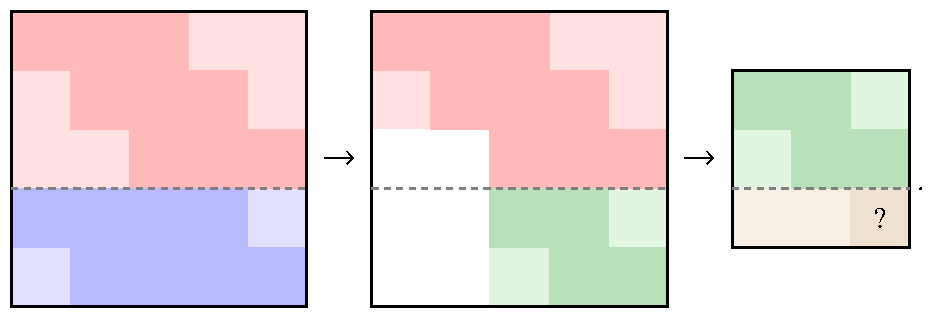
\includegraphics[width=0.8\textwidth]{papers/resultante/pictures/FinalTableau.pdf}
    \label{resultante:equation:finalTab}
\end{equation*}
Falls der letzte Rest im braunen Feld \(\neq0\) übrig bleibt, ist
der grösste gemeinsame Teiler \(=1\), die beiden Polynome \(a(X)\)
und \(b(X)\) sind somit teilerfremd.

Daraus lässt sich ablesen, dass die Determinante genau dann von Null
verschieden ist, wenn die beiden Polynome teilerfremd sind.
\begin{satz}[Resultante und Teiler]
    Zwei Polynome \(f(X)\) und \(g(X)\) sind genau dann teilerfremd,
    wenn \(\det(\syl(f,g))\neq0\) ist.
\end{satz}
\begin{definition}[Resultante]
    Wie bereits in der Einleitung
    (Abschnitt~\ref{resultante:equation:definition})
    geschrieben: Sind \(f\) und \(g\) Polynome, dann heisst die Determinante
    der Sylvester-Matrix
    \begin{equation*}
        \Res(f,g)=\det(\syl(f,g))
    \end{equation*}
    die \emph{Resultante} der Polynome.
    \label{resultante:definition:resultante}
\end{definition}

Folglich ist die Resultante zweier Polynome genau dann gleich Null,
wenn sie eine gemeinsame Nullstelle haben.

Das Beispiel \ref{resultante:beispiel:ggt} zeigt: Die Berechnung der
Resultante lässt sich bereits mit grund\-legenden Werkzeugen der linearen
Algebra umsetzen.

%
% 3_Resultante.tex -- Abschnitt 3 Resultante 
%
% (c) 2026 Jakob Gierer, OST Ostschweizer Fachhochschule
%
% !TEX root = ../../buch.tex
% !TEX encoding = UTF-8
%
\section{Resultante
\label{resultante:section:resultante}}
\kopfrechts{Resultante}

Die Resultante ist ein Werkzeug der CAS, um das Vorhandensein gemeinsamer
Nullstellen zweier Polynome zu prüfen.
Die Resultante kann ebenfalls dazu verwendet werden, die Variablen eines
Gleichungssystems mit mehreren Variablen zu eliminieren.
Zu diesem Zweck wurde die Resultante im 19.~Jahrhundert untersucht
\cite{resultante:resultante}.
% In modernen CAS werden Resultanten unter anderem benutzt, um aus einer vorher bestimmten Gröbner-Basis auf die Lösung eines Gleichungssystems zu schliessen. 

\subsubsection{Nützliche Eigenschaften
\label{resultante:subsubsection:eigenschaften}}

Die Resultante bietet einige nützliche Eigenschaften.
Die erste und relevanteste Eigenschaft für dieses Kapitel ist, dass
die Resultante gemeinsame Nullstellen findet.
Zusätzlich dazu bietet sie auch einen Weg zur parametrischen Berechnung
der Nullstellen.

Wie bereits in (\ref{resultante:equation:detsyl}) gezeigt, ist die
Resultante bis auf ein Vorzeichen symmetrisch:
\begin{equation*}
    \Res(f,g)=(-1)^{mn}\Res(g,f).
\end{equation*}
Insbesondere wenn \(mn\) gerade ist, sind die beiden Resultanten gleich.
\index{Symmetrie}%

Eine weitere wichtige Eigenschaft ist die Elimination von Variablen,
was in der Anwendung in (\ref{resultante:equation:resz}) ebenfalls
genutzt wird.
\begin{beispiel}
    Die Elimination von Variablen wird am Beispiel der Polynome
    \(f(x,y)=x^2+xy+1\) und \(g(x,y)=x-y\) gezeigt.
    Hier treten nun zwei Unbekannte auf: \(x\) und \(y\).
    Für die Aufstellung der Resultante bedeutet dies, dass es zwei
    Möglichkeiten gibt, die Polynome und die Resultante zu betrachten:
    \begin{enumerate}
        \item Als Polynom in \(x\) mit Koeffizienten, die \(y\) enthalten
            \begin{equation*}
\def\l#1{\bgroup\color{gray!20}#1\egroup}
                \begin{aligned}
                    \Rightarrow\quad&\begin{minipage}[t]{8cm}\raggedright
                                $x$ wird zum ``Einsortieren'' der Koeffizienten
                                in der Sylvester-Matrix verwendet und somit
                                eliminiert.
                                \end{minipage}\\
                    \Rightarrow\quad& \Res_x(f,g)=
                    \det
                    \begin{pmatrix}
                        1 & \phantom{-}y & \phantom{-}1\\
                        1 & -y & \phantom{-}\l{0}\\
                        \l{0} & \phantom{-}1 & -y
                    \end{pmatrix}
                    =2y^2+1.
                \end{aligned}
            \end{equation*}
        \item Als Polynom in \(y\) mit Koeffizienten, die \(x\) enthalten
            \begin{equation*}
                \begin{aligned}
                \Rightarrow\quad& \Res_y(f,g)=
                \det
                \begin{pmatrix}
                    \phantom{-}x & x^2+1\\
                    -1 & x
                \end{pmatrix}
                =2x^2+1.
		\end{aligned}
\qedhere
            \end{equation*}
    \end{enumerate}
    % \kreis{1} Als Polynom in \(x\) mit Koeffizienten, die \(y\) enthalten
    % \begin{equation*}
    %     \begin{aligned}
    %         &\Longrightarrow x \phantom{x} \text{wird zum ``einsortieren'' der Koeffizienten in der }\\
    %         &\hspace{21pt}\text{Sylvester-Matrix verwendet und somit eliminiert.}\\
    %         &\Longrightarrow \Res_x(f,g)=\det(\syl_x(f,g))=2y^2+1
    %     \end{aligned}
    % \end{equation*}
    % \kreis{2} Als Polynom in \(y\) mit Koeffizienten, die \(x\) enthalten
    % \begin{equation*}
    %     \Longrightarrow \Res_y(f,g)=\det(\syl_y(f,g))=2x^2+1.
    % \end{equation*}
    \label{resultante:beispiel:elimination}
\end{beispiel}
\noindent
Das tiefgestellte \(x\) oder \(y\) gibt dabei an, nach welcher Resultante aufgelöst wird.
Dabei verschwindet diese Variable aus dem Resultanten-Polynom (\(R(y)=\Res_x(f,g)=2y^2+1\)).

Die Resultante liegt im von \(f\) und \(g\) erzeugten Ideal, das man als \((f,g)\) schreibt, also
\begin{equation}
    \Res(f,g) \in (f,g).
\end{equation}
Das bedeutet, es existieren Polynome \(s(X)\) und \(t(X)\), daraus folgt:
\begin{equation}
    \Res(f,g) = s(X)f(X)+t(X)g(X).
    \label{resultante:equation:kombi}
\end{equation}
Im Prinzip ähnelt dies dem Span aus der linearen Algebra.
Bei Vektoren ist
\begin{equation}
    \Span(v_1,v_2)=av_1+bv_2,
\end{equation}
wobei \(a\), \(b\) Zahlen sind.
Beim Ideal \((f,g)\) dürfen die Faktoren \(s\), \(t\) selbst Polynome sein.

\begin{beispiel}
    Am Beispiel von \(f(X)=X-2\) und \(g(X)=X-5\) wird gezeigt:
    Die Resultante aus diesen Polynomen ist
    \begin{equation*}
        \Res(f,g)=\det
        \begin{pmatrix}
            1 & -2\\
            1 & -5
        \end{pmatrix}
        =-3.
    \end{equation*}
    Dabei ist
    \begin{equation*}
        -1\cdot f+ 1\cdot g=-3,
    \end{equation*}
    mit den Polynomen \(s(X)=-1\) bzw. \(t(X)=1\) und deshalb
    \begin{equation*}
        \Res(f,g)\in(f,g). \qedhere
        \label{resultante:equation:ideal}
    \end{equation*}
    \label{resultante:beispiel:ideal}
\end{beispiel}

Eine ähnliche Form zu (\ref{resultante:equation:kombi}) erhält man
durch den erweiterten euklidischen Algorithmus.
Aus dieser Form lässt sich ein effizientes Berechnungsverfahren für
die Resultante ableiten, das Subresultanten-Verfahren
(siehe Abschnitt~\ref{resultante:section:fortsetzung}).
\index{Subresultanten-Verfahren}%

%
% 4_RothsteinTrager.tex -- Abschnitt 4 Resultante anwendung in RT
%
% (c) 2026 Jakob Gierer, OST Ostschweizer Fachhochschule
%
% !TEX root = ../../buch.tex
% !TEX encoding = UTF-8
%
\section{Der Satz von Rothstein-Trager
\label{resultante:section:RT}}
\kopfrechts{Der Satz von Rothstein-Trager}
In der Anlaysis verwendet man für die Berechnung von Stammfunktionen
bei Integralen die Partialbruchzerlegung.
Bei dieser Methode müssen die Nullstellen des Nennerpolynoms bekannt sein.
Das Problem ist also, die Residuen des Integranden zu berechnen, ohne
\index{Residuum}%
den Nenner zu faktorisieren.
Die Mathematiker Rothstein und Trager haben unabhängig voneinander den
\index{Rothstein-Trager}%
Satz \ref{resultante:satz:RT} bewiesen.
Der rationale Teil \(a(z)\) muss teilerfremd zu \(b(z)\) sein, mit \(\deg
(a)<\deg (b)\).
Zusätzlich dazu muss das Polynom \(b(z)\) quadratfrei sein, dann sagt
das Liouville-Prinzip die Form
\index{Liouville-Prinzip}%
\begin{equation*}
    \int\frac{a(z)}{b(z)}\,dz=\sum_{k=1}^{m}c_k\log v_k(z)
    \label{resultante:equation:satzRT}
\end{equation*}
der Stammfunktion voraus. Gesucht sind nun die \(c_k\), für die
\begin{equation}
    a(z)-c_k\cdot b'(z) \quad \text{und} \quad b(z)
    \label{resultante:equation:polynome}
\end{equation}
einen nitchttrivialen grössten gemeinsamen Teiler (Teiler \(\neq1\))
\begin{equation}
    v_k(z)=\ggt\left(a(z)-c_k\cdot b'(z),b(z)\right)
    \label{resultante:equation:vks}
\end{equation}
haben.

\begin{satz}[Rothstein-Trager]
\index{Rothstein-Trager, Satz von}%
\index{Satz!von Rothstein-Trager}%
    Die Nullstellen von \(R(c)\) sind genau die Residuen von
\index{Residuum}%
    \(\frac{a(z)}{b(z)}\).
    \label{resultante:satz:RT} 
\end{satz}
\noindent
Die Nullstellen von \(R(c)=\Res_z(a-c\cdot b',b)\) sind die gesuchten \(c_k\).

Dafür eignet sich die Resultante nach Definition
\ref{resultante:definition:resultante} hervorragend.
Sie liefert als Lösung direkt den \(\ggt\) zweier Polynome mit
dazugehöriger Nullstelle.

\subsection{Anwendung der Resultante
\label{resultante:subsection:anwendung}}
Für die Bestimmung der Nullstellen \(c_k\) und des grössten gemeinsamen
Teilers \(v_k(z)\) wird die Resultante
\begin{equation}
    R(c)
    =
    \Res_z\left(a(z)-c\cdot b'(z),b(z)\right)%=0
    \label{resultante:equation:resz}
\end{equation}
benötigt.
In der Resultante \(R(c)\) wird die Variable \(z\) wie in Beispiel
\ref{resultante:beispiel:elimination} eliminiert.
Gesucht sind dann die Nullstellen $c_k$ mit \(R(c_k)=0\).

\begin{beispiel}
    Die Stammfunktion von
\index{Stammfunktion}%
    \begin{equation*}
        \int\frac{1}{z^3+z}\,dz
    \end{equation*}
    soll mit der Methode von Rothstein-Trager und der Resultante bestimmt
    werden.
    Die Bedingungen für die Rothstein-Trager-Methode sind bereits
    erfüllt mit \(a(z)=1\) und \(b(z)=z^3+z\).
    Es müssen daher die \(c_k\) und die dazugehörigen \(v_k(z)\)
    gefunden werden.
    Für die Resultante braucht es
    \begin{equation}
        \begin{aligned}
            a(z)&=1\\
            b(z)&=z^3+z\\
            b'(z)&=3z^2+1,
        \end{aligned}
        \label{resultante:equation:factoren}
    \end{equation}
    sie sieht wie folgt aus:
    \begin{equation}
        \Res_z\left(-3cz^2+1-c,z^3+z\right)=0.
        \label{resultante:equation:resZgut}
    \end{equation}
    Die daraus folgende Sylvester-Matrix ist:
    \begin{equation}
\def\l#1{\bgroup\color{gray!20}#1\egroup}
        \begin{NiceArray}{*{5}{c}}[cell-space-limits=3pt]
        -3c   & 0     & 1-c & \l{0} & \l{0} \\
        \l{0} & -3c   & 0   & 1-c   & \l{0} \\
        \l{0} & \l{0} & -3c & 0     & 1-c   \\
        1     & 0     & 1   & 0     & \l{0} \\
        \l{0} & 1     & 0   & 1     & 0
        \CodeAfter
            \tikz {
                \draw ([xshift=-3pt,yshift=1pt]1-|1) rectangle ([xshift=4pt,yshift=-1pt]6-|6);
                \draw[dashed] ([xshift=-3pt,yshift=1pt]4-|1) -- ([xshift=4pt,yshift=1pt]4-|6);
            }
        \end{NiceArray}
        \;\to\;
        \begin{NiceArray}{*{5}{c}}[cell-space-limits=3pt]
        \;1\;     & \;0\; & \frac{c-1}{3c} & \l{0}          & \l{0} \\
        \l{0} & 1     & 0              & \frac{c-1}{3c} & \l{0} \\
        \l{0} & \l{0} & 1              & 0              & \frac{c-1}{3c} \\
        1     & 0     & 1              & 0              & \l{0} \\
        \l{0} & 1     & 0              & 1              & 0
        \CodeAfter
            \tikz {
                \draw ([xshift=-4pt,yshift=1pt]1-|1) rectangle ([xshift=3pt,yshift=-1pt]6-|6);
                \draw[dashed] ([xshift=-4pt,yshift=0.5pt]4-|1) -- ([xshift=3pt,yshift=0.5pt]4-|6);
            }
        \end{NiceArray}\,\,\,.
        \label{resultante:equation:sylGutStep1}
    \end{equation}
    Nach Anwendung der Zeilenoperationen erhält man das erste Tableau.
    Auf dem kleineren Bereich kann nochmals eine Zeilenoperation
    durchgeführt werden:
    \begin{equation}
\def\l#1{\bgroup\color{gray!20}#1\egroup}
        \begin{NiceArray}{*{5}{c}}[cell-space-limits=3pt]
        \;1\; & \,\;0\;\, & \frac{c-1}{3c}  & \l{0}           & \l{0} \\
        \l{0} & 1         & 0               & \frac{c-1}{3c}  & \l{0} \\
        \l{0} & \l{0}     & 1               & 0               & \frac{c-1}{3c}\\
        \l{0} & \l{0}     & \frac{2c+1}{3c} & 0               & \l{0} \\
        \l{0} & \l{0}     & \l{0}           & \frac{2c+1}{3c} & 0
        \CodeAfter
            \tikz {
                \draw ([xshift=-4pt,yshift=1pt]1-|1) rectangle ([xshift=3pt,yshift=-1pt]6-|6);
                \draw[dashed] ([xshift=1pt]3-|3) -- ([xshift=1pt,yshift=-1pt]6-|3);
                \draw[dashed] ([xshift=1pt]3-|3) -- ([xshift=3pt]3-|6);
                \draw[dashed] ([xshift=1pt]4-|3) -- ([xshift=3pt]4-|6);
            }
        \end{NiceArray}
        \;\to\;
        \begin{NiceArray}{*{3}{c}}[cell-space-limits=3pt]
        \,1\, & \;0\; & \l{0}         \\
        \l{0} & 1     & 0             \\
        \l{0} & \l{0} & \frac{c-1}{3c}
        \CodeAfter
            \tikz {
                \draw ([xshift=-3pt,yshift=1pt]1-|1) rectangle ([xshift=3pt,yshift=-1pt]4-|4);
                \draw[dashed] ([xshift=-3pt]3-|1) -- ([xshift=3pt]3-|4);
            }
        \end{NiceArray}\,\,\,.
        \label{resultante:equation:sylGutStep2}
    \end{equation}
    Das Schlusstableau hat als entscheidendes Element:
    \begin{equation}
        \begin{aligned}
            \frac{c-1}{3c}&\overset{!}{=}0\\
            c_1&=1,
        \end{aligned}
        \label{resultante:equation:solGut1}
    \end{equation}
    für \(c_1=1\) lässt sich im Schlusstableau aus
    (\ref{resultante:equation:sylGutStep2}) für \(v_1(z)\) der \(\ggt=z\)
    ablesen.
    Findige Leser konnten bereits im vorherigen Tableau aus
    (\ref{resultante:equation:sylGutStep2}) den Algorithmus beenden,
    nämlich mit:
    \begin{equation}
        \begin{aligned}
            \frac{2c+1}{3c}&\overset{!}{=}0\\
            2c+1&=0\\
            2c&=-1\\
            c_2&=-\frac{1}{2},
        \end{aligned}
        \label{resultante:equation:solGut2}
    \end{equation}
    für \(c_2=-\frac{1}{2}\) lässt sich ebenfalls im zweitletzten
    Tableau aus (\ref{resultante:equation:sylGutStep2}) für \(v_2(z)\)
    der \(\ggt=z^2+1\) ablesen.

    Setzt man die gefundenen Nullstellen mit ihrem jeweils zugehörigen
    grössten gemeinsamen Teiler zusammen, erhält man die Stammfunktion:
    \begin{equation*}
        \int\frac{1}{z^3+z}\,dz=c_1\log v_1(z)+c_2\log v_2(z)
        =
        1\log z-\frac{1}{2}\log(z^2+1). \qedhere
    \end{equation*}
    \label{resultante:beispiel:gutesIntegral}
\end{beispiel}

\begin{beispiel}
    Die Methode soll mit einem weiteren Beispiel verdeutlicht werden.
    Das Integral
    \begin{equation*}
        \int\frac{1}{\log x}\,dx
    \end{equation*}
    soll gelöst werden.
    Dafür muss \(F(\vartheta)=\mathbb{Q}(x)\) mit dem logarithmischen
    Element \(\vartheta=\log x\) erweitert werden.
    Der Integrand wird dadurch zu
    \begin{equation*}
        f=\frac{1}{\vartheta}
    \end{equation*}
    mit
    \begin{equation}
        \begin{aligned}
            a(\vartheta)&=1\\
            b(\vartheta)&=\vartheta\\
            Db(\vartheta)&=\frac{1}{x}.
        \end{aligned}
    \end{equation}
    Das \(D\) steht hier für die Derivation nach \(x\).
    Die Resultante daraus sieht wie folgt aus:
    \begin{equation}
        R(c)
        =
        \Res_\vartheta(a(\vartheta)-cDb(\vartheta),b(\vartheta))
        =
        \Res_\vartheta\biggl(1-c\frac{1}{x},\vartheta\biggr)=0,
        \label{resultante:equation:resTbad}
    \end{equation}
    das erste Polynom in der Resultante ist vom Grad \(0\) und das zweite
    vom Grad \(1\).
    Die daraus entstehende \(1\times1\)-Sylvester-Matrix im Tableau ist dann
    \begin{equation}
        \begin{NiceArray}{c}[cell-space-limits=3pt]
        1-c\frac{1}{x} \\
        \CodeAfter
            \tikz \draw ([xshift=-3pt,yshift=2pt]1-|1) rectangle ([xshift=3pt,yshift=-2pt]2-|2);
        \end{NiceArray}
        \,\,\,\,\,\,.
        \label{resultante:equation:sylBad}
    \end{equation}
    Der Algorithmus für dieses Tableau endet, bevor er überhaupt das
    erste Mal angewandt wird.
    Das kritische Element ist:
    \begin{equation}
        \begin{aligned}
            1-\frac{c}{x}&\overset{!}{=}0\\
            \frac{c}{x}&=1\\
            c&=x,
        \end{aligned}
        \label{resultante:equation:solBad}
    \end{equation}
    die Nullstelle \(c\) muss für die Methode von Rothstein-Trager eine
    Konstante sein (\(Dc\overset{!}{=}0\)).
    Hier ist
    \begin{equation*}
        Dc=Dx=1\overset{!}{=}0 \,\text{\lightning}
    \end{equation*}
    Daraus folgt: das Integral ist nicht elementar lösbar.
    Wie Beispiel \ref{buch:intalg:risch:bsp:1/logx} und Definition
    \ref{buch:intalg:risch:def:integrallogarithmus} zeigt, ist das der
    Integrallogarithmus.
    \label{resultante:beispiel:badIntegral}
\end{beispiel}

Sobald die Nullstellen \(c_k\) aus der Resultante keine Konstanten sind,
folgt daraus, dass solche Integrale nicht elementar lösbar sind.

%
% 5_Fortsetzung.tex -- Abschnitt 5 Fortsetzende Idee der Resultanten Berechnung
%
% (c) Jakob Gierer, OST Ostschweizer Fachhochschule
%
% !TEX root = ../../buch.tex
% !TEX encoding = UTF-8
%
\section{Geht das noch besser?
\label{resultante:section:fortsetzung}}
\kopfrechts{Polynom-Restfolgen}
Der euklidische Algorithmus zur Berechnung grösster gemeinsamer Teiler
zweier ganzer Zahlen ist mehr als 2000 Jahre alt.
\index{euklidischer Algorithmus}%
Es ist der älteste bekannte Algorithmus.
Beim Versuch, den euklidischen Algorithmus zu verallgemeinern, um den
grössten gemeinsamen Teiler oder die Resultante von zwei Polynomen
zu berechnen, erreicht man schnell das Konzept der Polynom-Restfolge
(polynomial remainder sequence, PRS).
Dies führt zu schnell anwachsenden Koeffizienten.
Dieses schnelle Anwachsen ist zum Glück nicht Teil des Problems, sondern
ein Artefakt der naiven Ansätze der Verallgemeinerung.
Das Wachstum lässt sich kontrollieren, indem von jedem Polynom der PRS
ein nicht benötigter Teil entfernt wird.
Was dieser Teil ist und wie er entfernt wird, erschliesst sich im
folgenden Abschnitt.

Der Schlüssel, um dieses Koeffizienten-Wachstum zu kontrollieren,
ohne die aufwendige Berechunug des \(\ggt\) der Koeffizienten, ist die
Grundlage der Subresultanten.
Das Theorem von Subresultanten aus \cite{resultant:PRSalg} zeigt, dass
\index{Subresultante}%
jedes Polynom einer PRS proportional zu einer Subresultanten der ersten
zwei Polynome dieser Folge ist.


\subsection{Grundlegender Aufbau
\label{resultante:subsection:aufbau}}
Für die Konstruktion einer PRS wird die Division mit Rest benötigt,
dabei kann dies beliebig normiert werden.
Der euklidische Algorithmus teilt zwei Polynome in \(\mathbb{Q}\),
wobei das Polynom mit dem grösseren Grad der Dividend ist und das mit
dem kleineren der Divisor:
\begin{equation}
    P_i / P_{i+1} = Q_i \quad \text{mit}\quad R_i.
\end{equation}
Als nächster Schritt wird der Rest \(R_i\) der Division zum neuen Divisor
\(P_{i+2}\) und der alte Divisor wird zum neuen Dividend \(P_{i+1}\).
Durch die Division können problematische Brüche als Koeffizienten entstehen.
\begin{beispiel}
    Mit den Polynomen \(a(X)=4X^4-7X^3+22X^2-24X+5\) und
    \(b(X)=8X^3+8X^2-16X\) soll der euklidische Algorithmus gezeigt
    werden.
    Begonnen wird mit \(P_1=a(X)\) und \(P_2=b(X)\), da
    \(\deg(a)>\deg(b)\) ist, dabei wird
    \begin{equation}
        (4X^4-7X^3+22X^2-24X+5)/(8X^3+8X^2-16X).
    \end{equation}
    Nach der Polynom-Division erhählt man
    \(Q_1=\frac{X}{2}-\frac{11}{8}\) und \(R_1=P_3=41X^2-46X+5\).
    Die nächste Division ist
    \begin{equation*}
        P_2/P_3,
    \end{equation*}
    daraus folgt die neue Division
    \begin{equation}
        (8X^3+8X^2-16X)/(41X^2-46X+5),
    \end{equation}
    was \(R_2=P_4=\frac{3480}{1681}X-\frac{3480}{1681}\) ergibt.
    Da \(R_2\neq0\) ist, geht der Algorithmus weiter mit
    \begin{equation*}
        P_3/P_4,
    \end{equation*}
    und
    \begin{equation}
        (41X^2-46X+5)\Big/\biggl(\frac{3480}{1681}X-\frac{3480}{1681}\biggr),
    \end{equation}
    daraus resultiert \(R_3=P_5=0\).
    \label{resultante:beispiel:eualg}
\end{beispiel}
Wie man in Beispiel \ref{resultante:beispiel:eualg} sieht, entstehen
bei der Division grosse Brüche.
Zudem ist der Grad jedes weiteren Polynoms um eins kleiner als der
des vorherigen.

\subsection{Verbesserungsmöglichkeiten
\label{resultante:subsection:besser}}
Der euklidische Algorithmus liefert eine Folge von Quotienten und Resten.
Diese Quotienten und Reste führen in der Standardvorgehensweise zu
Brüchen, deren Zähler und Nenner riesig werden können.
Dies ist der Grund für die verallgemeinerte PRS, mit den folgenden
Zielen zur Optimierung:
\begin{enumerate}[label=\alph*)]
    \item Rechnen nur mit ganzen Zahlen, da dies effizienter ist (kein
    Kürzen von Brüchen).
    \item Nur mit kleinen Koeffizienten rechnen.
\end{enumerate}

\subsection{PRS für ganzzahlige Rechnung
\label{resultante:subsection:ganzzahlig}}
Angenommen, die Terme eines Polynoms \(P\) sind in absteigender Potenz
sortiert, dann ist der Koeffizient des ersten Terms der Leitkoeffizient
\(\lc(P)\).
\index{Leitkoeffizient}%
\index{lc(P)@$\operatorname{lc}(P)$}%
Daher kann man die normale Division und deren Rest durch eine neue
Pseudo-Division mit Pseudo-Rest ersetzen, in der sich die Resultate
\index{Pseudo-Division}%
\index{Pseudo-Rest}%
der normalen Divison und der normale Rest nur um bestimmte Faktoren
unterscheiden.
Die Pseudo-Division hat rein ganzzahlige Pseudo-Quotienten
\(Q=\pquo(f,g)\) mit ganzzahligem Pseudo-Rest \(R=\prem(f,g)\).
Anders als in der gewöhlichen Polynom-Division mit Rest entstehen dabei
keine Brüche, da mit einer Potenz des Leitkoeffizienten des Divisors
multipliziert wird, sodass
\begin{equation}
    b_i^{\delta_i+1}P_i-Q_iP_{i+1}=R_i \quad \text{und} \quad \deg(R)<\deg(P_{i+1})\quad \text{für} \quad i=1,\dots,k-1 \, \text{ist},
    \label{resultante:equation:algpdivi}
\end{equation}
wobei \(b_i\) der Leitkoeffizient von \(P_{i+1}\) (\(\lc(P_{i+1})\)),
\(\delta_i=\deg(P_i)-\deg(P_{i+1})\) und \(P_{i+2}=R_i\) ist.
Bei Anwendung derselben Vorgehensweise auf \(P_2\) und \(P_3\), und
danach auf \(P_3\) und \(P_4\) usw., entsteht eine Folge
\begin{equation}
    P_1,P_2,P_3,\dots,P_k,P_{k+1}=0.
    \label{resultante:equation:prs}
\end{equation}
Eine solche Folge heisst Polynom-Restfolge (PRS).
\index{Polynom-Restfolge}%
\index{polynomial remainder sequence}%
\index{PRS}%

\begin{beispiel}
    Aus den Polynomen \(a(X)=4X^4-7X^3+22X^2-24X+5\) und
    \(b(X)=8X^3+8X^2-16X\) soll die PRS gebildet werden.
    Begonnen wird mit \(P_1=a(X)\) und \(P_2=b(X)\), dabei ist
    \begin{equation*}
        b_1 = 8, \qquad \delta_1=4-3=1.
    \end{equation*}
    Aus (\ref{resultante:equation:algpdivi}) folgt im ersten Schritt
    \begin{equation}
        8^{1+1}P_1-Q_1P_2=R_1,
    \end{equation}
    nach der Pseudo-Division erhält man \(Q_1=32X-88\) und
    \(R_1=P_3=2624X^2-2944X+320\).
    Der nächste Schritt hat
    \begin{equation*}
        b_2 = 2624, \qquad \delta_2=2-1=1,
    \end{equation*}
    daraus folgt die neue Division
    \begin{equation}
        2624^{1+1}P_2-Q_2P_3=R_2,
    \end{equation}
    was \(Q_2=20992X+44544\) und \(R_2=P_4=14254080X-14254080\) ergibt.
    Da \(R_2\neq0\) ist, geht der Algorithmus weiter mit
    \begin{equation*}
        b_3 = 14254080, \qquad \delta_3=1-1=0,
    \end{equation*}
    und
    \begin{equation}
        14254080^{1}P_3-Q_3P_4=R_3,
    \end{equation}
    daraus resultiert \(Q_3=37402705920X-4561305600\) und \(R_3=P_5=0\).
    Die aus den Rest-Polynomen entstehende Folge ist
    \begin{align*}
            P_1&=4X^4-7X^3+22X^2-24X+5, \\
            P_2&=8X^3+8X^2-16X, \\
            P_3&=2624X^2-2944X+320, \\
            P_4&=14254080X-14254080, \\
            P_5&=0.
	\qedhere
    \end{align*}
    \label{resultante:beispiel:prs}
\end{beispiel}
Wie man in Beispiel \ref{resultante:beispiel:prs} beobachten kann,
wird Ziel a) erreicht, aber b) völlig verfehlt.
Die Koeffizienten der PRS explodieren.
Ist das letzte Polynom der Folge \(P_{k+1}=0\), dann ist \(P_k\)
der unnormierte \(\ggt\), in Beispiel \ref{resultante:beispiel:prs}
\(P_4=14254080(X-1)\).


\subsection{Subresultanten-PRS
\label{resultante:subsection:subresprs}}
Um das Koeffizienten-Wachstum in den Griff zu bekommen, wird die Folge
mit \(\beta_i\) normiert.
Dadurch wird
\begin{equation}
    \beta_i P_i=\prem(P_{i-2},P_{i-1})\quad \text{für} \quad i=3,\dots,k+1.
    \label{resultante:equation:prsnorm}
\end{equation}
Nun muss nur noch ein geeigneter Faktor \(\beta_i\) gefunden werden,
dieser kann im Prinzip beliebig gewählt werden.
Je nach Wahl des \(\beta_i\) ist das Koeffizienten-Wachstum besser oder
schlechter kontrollierbar, oder es kann sichergestellt werden, dass die
Koeffizienten immer in \(\mathbb{Z}\) bleiben.

Der künstliche Faktor, der in der Pseudo-Division vorkommt, ist bereits
bekannt und kommt als Skalierungsfaktor \(\beta_i\) infrage.
Es ist nicht ganz einfach, einen solchen \(\beta_i\)-Faktor zu finden,
der das Ziel a) immer noch erreicht.
Dieser \(\beta_i\)-Faktor kann in der PRS wie folgt festgelegt werden.
Um eine PRS zu formulieren, sei \(p_i=\lc(P_i)\) und man wählt
\begin{equation}
    \begin{aligned}
        \beta_3&=(-1)^{\delta_1+1}\\
        \beta_i&=(-1)^{\delta_{i-2}+1}p_{i-2}h^{\delta_{i-2}}_{i-2}, \quad i=4,\dots,k+1,
    \end{aligned}
    \label{resultante:equation:beta}
\end{equation}
wobei die Hilfsfaktoren \(h_i\)
\begin{equation}
    \begin{aligned}
        h_2&=p_2^{\delta_1}\\
        h_i&=p_i^{\delta_{i-1}}h^{1-\delta_{i-1}}_{i-1}, \quad i=3,\dots,k
    \end{aligned}
    \label{resultante:equation:h}
\end{equation}
sind.
Das ist die Brown-Normierung.
\index{Brown-Normierung}%
W.~S.~Brown hat in \cite{resultant:PRSalg} die Subresultanten-PRS
\index{Brown, W.~S.}%
weiterentwickelt, die George E.~Collins bereits in
\index{Collins, George E.}%
\cite{resultant:Collins} beschreibt.

Daraus folgt die Subresultanten-PRS.
Die daraus konstruierte Subresultanten-PRS mit \(G_1=P_1,\,G_2=P_2,\,G_3,\dots,\,G_k\), wird mit
\begin{equation}
    \begin{aligned}
        G_3&=(-1)^{\delta_1+1}\prem(G_1,G_2),\\
        G_i&=\frac{(-1)^{\delta_{i-2}+1}\prem(G_{i-2},G_{i-1})}{g_{i-2}h^{\delta_{i-2}}_{i-2}},\quad i=4,\dots,k+1
    \end{aligned}
    \label{resultante:equation:algsubprs}
\end{equation}
berechnet.
Die Iteration stoppt, sobald \(\prem(G_{k-1},G_k)=0\) ist.
Dann ist
\begin{equation}
    \ggt(P_1,P_2)=\pp(G_k), \qquad \Res(P_1,P_2)=0,
    \label{resultante:equation:ggtres}
\end{equation}
wobei \(\pp\) das primitive Polynom ist, im Beispiel
\ref{resultante:beispiel:prs} ist \(\pp(P_4)=X-1\).
Dabei haben die Koeffizienten den \(\ggt=1\).
Der Algorithmus soll mit folgendem Beispiel verdeutlicht werden.

\begin{beispiel}
    Zunächst wird mit \(G_1=P_1=a(X)=4X^4-7X^3+22X^2-24X+5\) und \(G_2=P_2=b(X)=8X^3+8X^2-16X\) begonnen.
    Für die Bestimmung von \(G_3\) wird nach (\ref{resultante:equation:algsubprs}) mit
    \begin{equation*}
        G_3=(-1)^{\delta_1+1}\prem(G_1,G_2)
    \end{equation*}
    begonnen, dabei ist
    \begin{equation*}
        \delta_1=\deg(G_1)-\deg(G_2)=1.
    \end{equation*}
    Daraus folgt
    \begin{equation*}
        G_3=\prem(G_1,G_2)=2624X^2-2944X+320.
    \end{equation*}
    Als nächstes wird \(G_4\) mit
    \begin{equation*}
        G_4=\frac{(-1)^{\delta_2+1}\prem(G_2,G_3)}{g_2h^{\delta_2}_2}
    \end{equation*}
    bestimmt, dafür braucht es
    \begin{equation*}
        \delta_2=\deg(G_2)-\deg(G_3)=1, \quad g_2=8, \quad h^{\delta_2}_2=g^{\delta_2}_2=8.
    \end{equation*}
    Das in die Gleichung für \(G_4\) eingesetzt ergibt
    \begin{equation*}
        G_4=\frac{\prem(G_2,G_3)}{8\cdot8}=222720X-222720.
    \end{equation*}
    Da \(G_4\neq0\) ist, geht der Algorithmus weiter mit
    \begin{equation*}
        G_5=\frac{(-1)^{\delta_3+1}\prem(G_3,G_4)}{g_3h^{\delta_3}_3}.
    \end{equation*}
    Hier müssen \(\delta_3, g_3, h_3\) nicht mehr bestimmt werden, da bereits \(\prem(G_3,G_4)=0\) ist und somit \(G_5=0\).
    Daraus entsteht die Subresultanten-PRS
    \begin{equation*}
        \begin{aligned}
            G_1&=4X^4-7X^3+22X^2-24X+5, \\
            G_2&=8X^3+8X^2-16X, \\
            G_3&=2624X^2-2944X+320, \\
            G_4&=222720X-222720, \\
            G_5&=0.
        \end{aligned}
    \end{equation*}
    Der \(\ggt\) ist nach (\ref{resultante:equation:ggtres}) links \(\ggt(P_1,P_2)=\pp(G_4)=X-1\).
    \label{resultante:beispiel:subprs}
\end{beispiel}
Wenn man \(P_4\) aus der gewöhlichen PRS mit \(G_4\) aus der
Subresultanten-PRS vergleicht, ist ganz deutlich zu sehen, welchen
Einfluss die Brown-Normierung auf die Koeffizienten hat.
Die Koeffizienten in \(G_4\) sind deutlich kleiner als die von \(P_4\).
Ziel a) wird immer noch erreicht und man ist dem Ziel b) deutlich näher
gekommen.

\subsection{Anwendung der Subresultanten-PRS
\label{resultante:subsection:subprs}}
\begin{beispiel}
    Wie in Beispiel \ref{resultante:beispiel:gutesIntegral} soll die
    Stammfunktion von
    \begin{equation*}
        \int\frac{1}{z^3+z}\,dz
    \end{equation*}
    bestimmt werden.
    Dafür muss die Resultante (\ref{resultante:equation:resZgut})
    \begin{equation}
        R(c)=\Res_z\left(-3cz^2+1-c,z^3+z\right)
        \label{resultante:equation:resprs}
    \end{equation}
    berechnet werden. 
    Dies soll mit der Subresultanten-PRS durchgeführt werden.
    Damit man den Überblick über die einzelnen Faktoren der Berechnung
    behält, werden sie in einer Tabelle notiert.
    Die \(G_i\) werden nach (\ref{resultante:equation:algsubprs}) in
    \begin{equation*}
        \begin{NiceArray}{|c|l|c|c|c|c|}[cell-space-limits=3pt]
            \hline
            i & G_i & \delta_i & n_i & g_i & h_i \\
            \hline
            1 & z^3+z & 1 & 3 & 1 & - \\
            2 & -3cz^2+1-c & 1 & 2 & -3c & -3c \\
            3 & 3c(2c+1)z & 1 & 1
            & 9c^2(2c+1)^2
            & -27c^3(2c+1)^2 \\
            4 & (1-c)(2c+1)^2 & - & 0 & - & - \\
            \hline
        \end{NiceArray}
        \label{resultante:equation:tabsubprs}
    \end{equation*}
    berechnet.
    Dabei ist \(n_i\) der Grad von \(G_i\), \(g_i\) der Leitkoeffizient
    \(\lc(G_i)\) und \(h_i\) der Hilfsfaktor.
    Da \(G_4\) konstant bezüglich \(z\) ist, ist \(G_4\) die Resultante
    \(\Res_z\left(-3cz^2+1-c,z^3+z\right)\).
    Die Resultante soll \(\Res_z=0\) sein, das wird erreicht, wenn
    \(c_1=1\) oder \(c_2=-\frac{1}{2}\) ist.
    Nun kann der \(\ggt\) mit \(G_3\) der darüber liegenden Zeile
    bestimmt werden, für \(c_1=1\):
    \begin{equation}
        \begin{aligned}
            G_3(c_1)&=3c_1(2c_1+1)z=3\cdot1(2\cdot1+1)z=9z\\
            \Rightarrow\quad \ggt&=\pp\left(G_3(c_1)=9z\right)=z.
        \end{aligned}
    \end{equation}
    Analog gilt für \(c_2=-\frac{1}{2}\):
    \begin{equation}
        G_3(c_2)
        =
        3c_2(2c_2+1)z
        =
        3\cdot-\frac{1}{2}\biggl(2\cdot-\frac{1}{2}+1\biggl)z=0,
    \end{equation}
    Hier geschieht Besonderes: \(G_3\) wird ebenfalls Null, wenn \(c_2\)
    eingesetzt wird.
    Um den \(\ggt\) zu bestimmen, muss daher \(G_2\) in der
    darüberliegenden Zeile verwendet werden:
    \begin{equation}
        \begin{aligned}
            G_2(c_2)&=-3c_2z^2+1-c_2=-3\cdot-\frac{1}{2}z^2+1-\biggl(-\frac{1}{2}\biggr)=1.5z^2+1.5\\
            \Rightarrow\quad \ggt&=\pp\left(G_2(c_2)=1.5z^2+1.5\right)=z^2+1.
        \end{aligned}
    \end{equation}
    Setzt man wieder die gefundenen Nullstellen mit den dazugehörigen
    \(\ggt\) zusammen, erhält man die Stammfunktion:
    \begin{equation*}
        \int\frac{1}{z^3+z}\,dz=c_1\log v_1(z)+c_2\log v_2(z)=1\log z-\frac{1}{2}\log(z^2+1). \qedhere
    \end{equation*}
    \label{resultante:beispiel:subprsRT}
\end{beispiel}
Das Beispiel \ref{resultante:beispiel:subprsRT} zeigt einen
Algorithmus, mit dem dasselbe erreicht wird, wie in Beispiel
\ref{resultante:beispiel:gutesIntegral}: einen Weg, die Resultante zu
berechnen und die Nullstelle zweier Polynome zu finden.


\printbibliography[heading=subbibliography]
\end{refsection}
